\section{Active Sensing Experiment}
    \subsubsection*{Input Parameter Data Sets}
    10 Parameter data sets are made with differenet combinations of number of chirps and IQ rate. The other parameters are fixed. \\
    \vspace{-4mm}  
    \begin{figure}[!h]\raggedleft
    \hspace{15mm}
		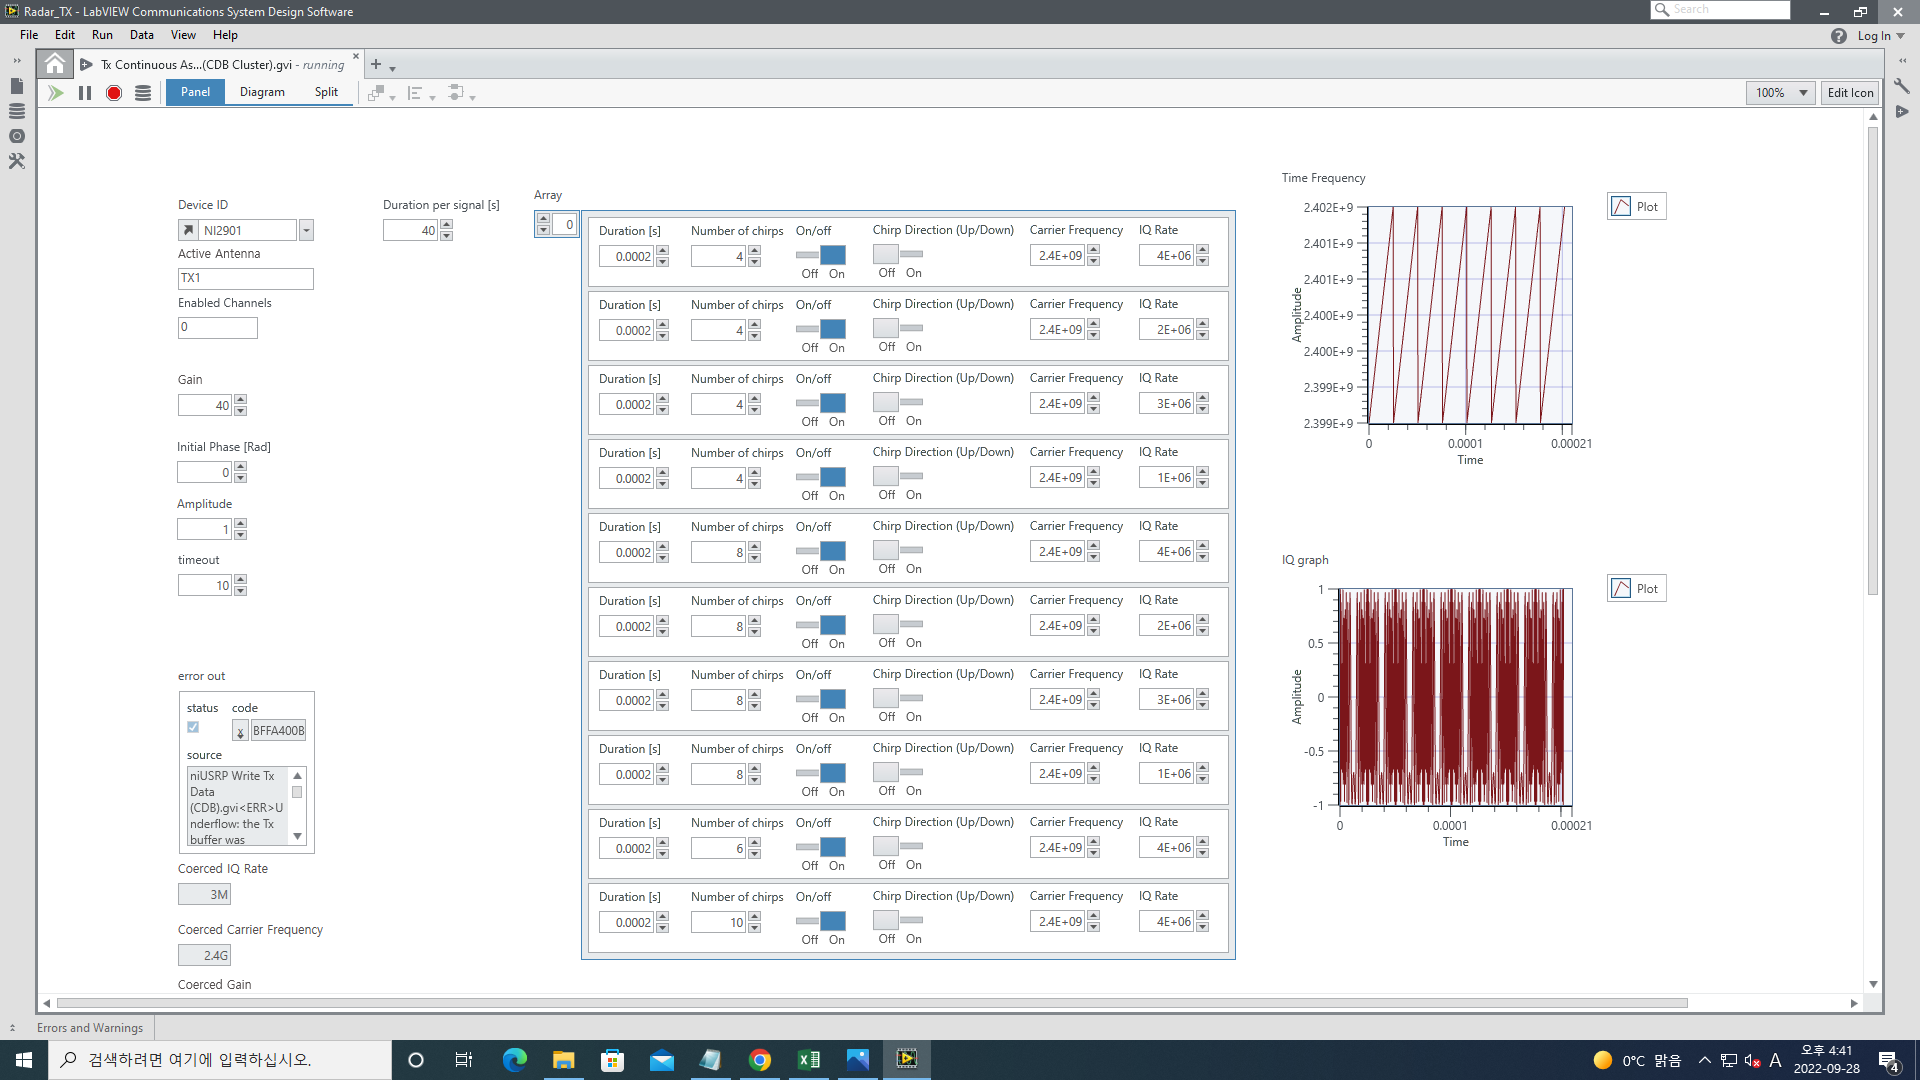
\includegraphics[width=.95\textwidth]{image/week04/1-1-b.png}
		\caption{\footnotesize TX panel}
		\vspace{-10pt}
    \end{figure}
    
    \begin{table}[!h]\centering
        \hspace{10mm}
        \begin{tabular}{|l|c|c|c|c|c|c|}
        \hline
        \multicolumn{1}{|l|}{Set} & 
        \multicolumn{1}{l|}{Duration} & 
        \multicolumn{1}{l|}{Number of Chirps} & 
        \multicolumn{1}{l|}{On} & 
        \multicolumn{1}{l|}{Chirp Direction} & 
        \multicolumn{1}{l|}{Carrier Frequency} & 
        \multicolumn{1}{l|}{IQ rate} \\
        \hline
        1 & 200u & 4 & on & off & 2.4G & 4M \\ 
        \hline
        2 & 200u & 4 & on & off & 2.4G & 2M \\ 
        \hline
        3 & 200u & 4 & on & off & 2.4G & 3M \\ 
        \hline
        4 & 200u & 4 & on & off & 2.4G & 1M \\ 
        \hline
        5 & 200u & 8 & on & off & 2.4G & 4M \\ 
        \hline
        6 & 200u & 8 & on & off & 2.4G & 2M \\ 
        \hline
        7 & 200u & 8 & on & off & 2.4G & 3M \\ 
        \hline
        8 & 200u & 8 & on & off & 2.4G & 1M \\ 
        \hline
        9 & 200u & 6 & on & off & 2.4G & 4M \\ 
        \hline
        10 & 200u & 10 & on & off & 2.4G & 4M \\ 
        \hline
        \end{tabular}
        \caption{Parameter Sets}
    \end{table}
\clearpage 
    
    \subsubsection*{Experiment Result}
    Executing Radar signal generator and Spectrum sensor, we could check the signal reception in the RX panel as below figure which used the parameter set 7. We can see the signal centered on 2.4GHz(Carrier Frequency) and has the bandwidth(IQ rate) of 3MHz. \\
    \vspace{-4mm}  
    \begin{figure}[!h]\raggedleft
    \hspace{15mm}
		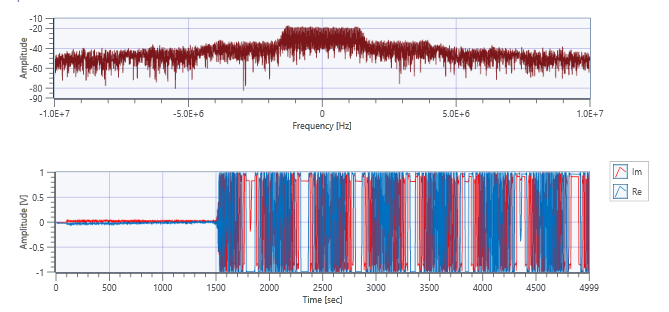
\includegraphics[width=.95\textwidth]{image/week04/1-1-0.png}
		\caption{\footnotesize RX panel}
		\vspace{-10pt}
    \end{figure}

    
    The IQ data is recorded in RX computer. Each csv file has 250us signal data with two columns, Imagainary and Real. \\
    \vspace{-4mm}  
    \begin{figure}[!h]\raggedleft
    \hspace{15mm}
		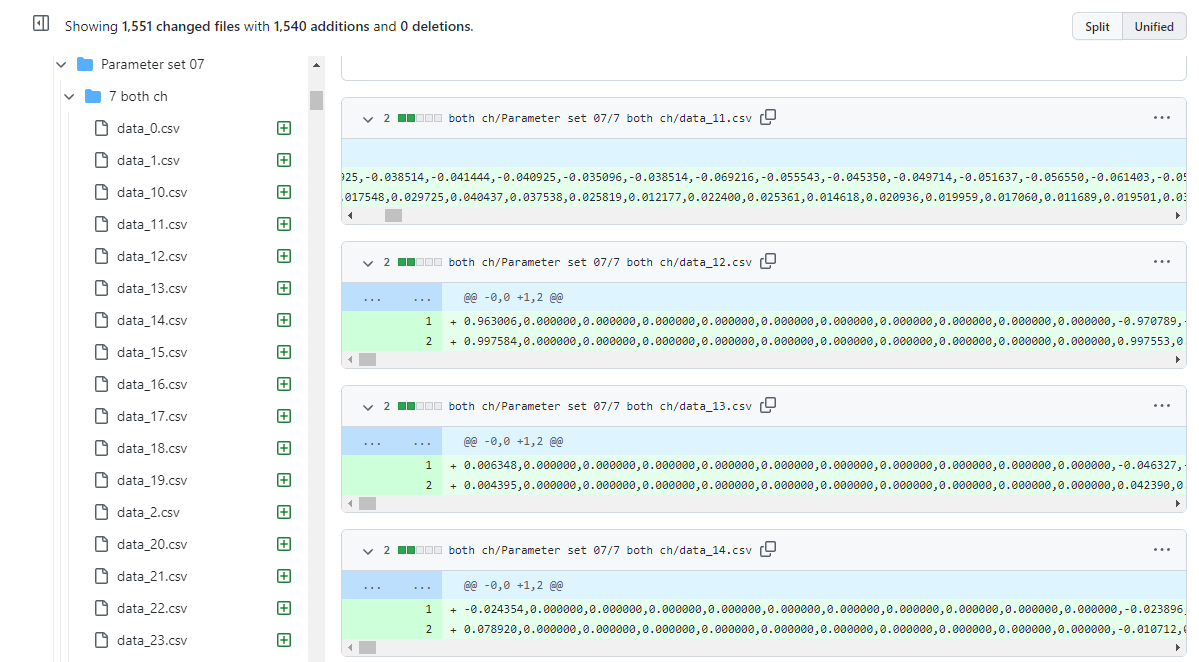
\includegraphics[width=.95\textwidth]{image/week04/1-1-a.png}
		\caption{\footnotesize IQ data}
		\vspace{-10pt}
    \end{figure}
    
\clearpage 
    \subsubsection*{Spectrograms}
    Using Python visualization code on IQ data of csv files, we generated spectrograms. The chirp signals appear in the middle of the spectrograms. As there was noise and interference, the chirp signals were received intermittently. The chirp signals seem more clear as the number of chirps decreases or IQ rate increases. \\
    \vspace{-4mm}  
    \begin{figure}[!h]\raggedleft
    \hspace{15mm}
		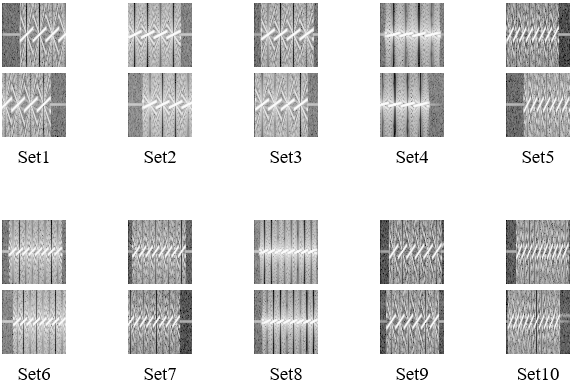
\includegraphics[width=.95\textwidth]{image/week04/1-1-1.png}
		\caption{\footnotesize Spectrograms, 10 sets}
		\vspace{-10pt}
    \end{figure}
    
    \subsubsection*{Discussion}
    Parameter sets 1, 9, 5, 10 differ in the number of chirps and the other parameters are fixed. Each of them has 4, 6, 8, 19 chirps. As the number of chirps increases, there are more chirps in one spectrogram and the slope of the chirp increases. \\
    
    \vspace{-4mm}  
    \begin{figure}[!h]\raggedleft
    \hspace{15mm}
		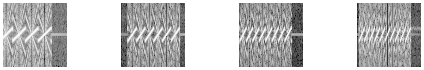
\includegraphics[width=.95\textwidth]{image/week04/1-1-2.png}
		\caption{\footnotesize Set 1, 9, 5, 10 : Number of Chirps 4, 6, 8, 10}
		\vspace{-10pt}
    \end{figure}
    
    Parameter sets 4, 2, 3, 1 / 8, 6, 7, 5 differ in IQ rate and the other parameters are fixed. Each of them has IQ rate of 1M, 2M, 3M, 4M. As IQ rate increases, the bandwidth increases and the slope of the chirp increases. \\
    
    \vspace{-4mm}  
    \begin{figure}[!h]\raggedleft
    \hspace{15mm}
		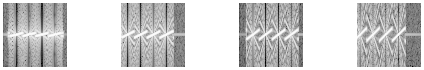
\includegraphics[width=.95\textwidth]{image/week04/1-1-3.png}
		\caption{\footnotesize Set 4, 2, 3, 1 : IQ rate 1M, 2M, 3M, 4M}
		\vspace{-10pt}
    \end{figure}
    
    \vspace{-4mm}  
    \begin{figure}[!h]\raggedleft
    \hspace{15mm}
		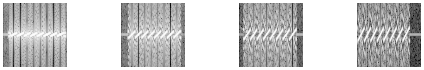
\includegraphics[width=.95\textwidth]{image/week04/1-1-4.png}
		\caption{\footnotesize Set 8, 6, 7, 5 : IQ rate 1M, 2M, 3M, 4M}
		\vspace{-10pt}
    \end{figure}
    
    

    %%%%%%%%%%%%%%%%%%%%%%%%%%%%%%%%%%%%%%%%%%%%%%%%%